\headline{{\textbf{\Large\sffamily Growing Together:}}\\
          {\textbf{\large\sffamily Bonsai Club News}}}
\phantomsection
\label{2026-01-news}
%\vfill

%\topic{Join the 2026 New Talent Competition}
%\noindent
%Are you ready to take your bonsai skills to the next level?
%The \textit{New Talent Competition (NTC)} is back for 2026, offering a unique platform for emerging enthusiasts to showcase their craft.
%This year's British heat takes place at \textit{Bonsai Fest in Newark on 22 March}.
%
%The winner will earn the prestigious opportunity to represent the UK at the European final in \textit{Slovakia on 11 April 2026}, with \textit{flights and accommodation fully covered}.
%
%To enter, you must be a non\--professional.
%Simply download the entry form at \href{https://fobbsbonsai.co.uk}{fobbsbonsai.co.uk} and return it by the \textit{30 January 2026 deadline}.
%For guidance and a formal referral, please speak to \textbf{Chris Durne or Nick Lloyd} at our next club meeting.

\topic{Support Bonsai Education – Donate Spare Tools!}
\noindent
\textbf{Brendan Gibbs and Mark Angold} are launching an exciting project to introduce bonsai to pupils at local schools --- one club at Brendan's school and another near Mark in Basingstoke. They've already sourced some trees from Corin Tomlinson (Greenwood Bonsai), and now they're looking for tools for the students to use during sessions.

If you have any spare or unused bonsai tools, or are planning to upgrade and have older ones to pass on, please consider donating them. Even general gardening tools would be greatly appreciated.

A donation box will be available at upcoming club nights for any contributions. Your support will help inspire the next generation of bonsai enthusiasts and ensure this wonderful initiative takes root!

% \begin{center}
% 	\includegraphics[width=0.5\columnwidth]{res/newspaper.png}
% \end{center}

% \topic{2025 Membership Renewal – Don't Forget!}
% \noindent
% Membership remains \textbf{£30} with monthly subs at \textbf{£5} for meetings at \emph{Whitton Community Centre} (extra sessions/external speaker nights may still incur additional costs). Payments can be made:
	
% \begin{itemize}
% 	\item \textbf{Online:} Twickenham Bonsai Club, A/C no. 53990897, Sort code 60-60-02 (please add a reference against the payment to help us identify where your payment has come from and log it via the Discord form as well).		
% 	\item \textbf{At the Next Meeting:} Cash or contactless.  
% \end{itemize}
	
% You can also prepay for the year's club nights—\textbf{12 sessions for £50 (10 months' price)}—bringing the total cost to \textbf{£80} for membership and subs.

\medskip	
\topic{Save on Club Merchandise with Shared Order!}
\noindent
The club's merchandise can be found at \url{https://overrock.uk/product-category/tw-bonsai/}. If you're thinking of making a purchase soon, reach out to Brendan on WhatsApp. Placing a shared order could help save a little on shipping costs.

\medskip
\topic{Bonsai Resources at Your Fingertips}
\noindent  
Our bonsai club is proud to offer a wide range of resources to help you grow and thrive in your bonsai journey. All these resources are conveniently organized on our Discord channel. If you're a subscribed member and haven't yet accessed the channel, simply \href{https://discord.gg/N6yka6XJ}{follow this link}.

Once you join, you'll land in the \href{https://discord.com/channels/873817545013071872/1118677826208550923}{welcome chat}. On the left\--hand side, you'll find a list of subchannels, each dedicated to a specific topic or service, such as \href{https://discord.com/channels/873817545013071872/1039691122148130876}{club payments}, \href{https://discord.com/channels/873817545013071872/1001189937409949698}{book recommendations}, and more. 

Whether you're a seasoned enthusiast or a new member, these resources are here to support your passion for bonsai. Don't miss out---get connected today!
%\columnbreak

\topic{Bonsai Insights: Information Pack for All Members}
\noindent
We've put together an information pack for all members of the club – from beginners to seasoned enthusiasts. This pack offers a wealth of resources, including access to a selection of our lockdown ZOOM talks featuring some of the best Bonsai artists in the country.

The following link will direct you to a Google slideshow \href{https://docs.google.com/presentation/d/1L5SRA_ZSvnGMLbRt0CSf-Uz7BaiOfxOs7OUHMM_XrTY/edit?usp=sharing}{New \& Existing Members Information Pack}, so feel free to explore it at your own pace. We recommend starting with Andy Hardman's talk on tree biology (Video 1), where he delves into how trees function and what they need to thrive.

% \medskip
% \topic{Don't Leaf Us Hanging: Meetup Time!}
% \noindent
% Come join us at 7pm on \textbf{11th September 2025} in the bar area at \emph{Whitton Community Centre, Percy Road, Whitton TW2 6JL}. Branching out, the subject of next \textbf{Tree of the Month} display will be \textbf{Evergreen}---bring your best!
	
% \topic{TWBC Winter Show 2025!}
% \noindent
% Our first show of the year is fast approaching! Please come along early to help setup the display and help the organisation during the day. Thanks in advance! See you on \textbf{Sunday, 2nd February 2025} at \emph{St Richard Reynolds Catholic College, Clifden Road, Twickenham, TW1 4LT}! 
	
% \topic{Grafting Workshop – Express Interest Now!}
% \noindent
% Steve will lead a workshop in March on grafting \textbf{Paul's Scarlet Hawthorn} onto regular hawthorn rootstock. Plants will be provided (limited availability). The workshop will cost \textbf{£5} and take place during the March club night. Contact Steve via WhatsApp to secure your spot. 

\closearticle
\columnbreak


\headline{{\textbf{\Large\sffamily Potting Shed Gossip:}}\\
          {\textbf{\large\sffamily Planting Seeds for the Future}}}
\label{2026-01-gossip}
\noindent
There is an old proverb that says, ``The best time to plant a tree was 20 years ago.
The second best time is now.''
This month, two of our own members, \textbf{Mark Angold} and {Brendan Gibbs}, took that sentiment to heart by officially launching a brand\--new bonsai school for children.
%
For months, our club has been quietly collecting second\--hand tools, wire, and pots, knowing they were destined for a special project.
Last week, that vision became a reality.
The first session was a resounding success, and the energy in the room was palpable.

\topic{``Proper Chuffed''}
\noindent
Brendan shared the exciting news with the club immediately after the session: \textit{``School session 1 completed! The kids loved it and are proper chuffed with their trees!''}
The outpouring of support from our members was instant, with Mark adding, \textit{``Oh gosh! That has absolutely made my year!''}

The impact of their hard work---all donated in their own free time---is perhaps best captured by a letter from Maria's parents, one of the new students:

\begin{quote}
    \textit{``The club is such a brilliant and interesting idea.}
    \textit{A wonderfully creative, mindful, and original outlook for young people who might be weighed down with negative distractions and worries.}
    \textit{We think you're fabulous for trialling it.''}
\end{quote}

\topic{Cultivating the Next Generation}
In the photos from the day, you can see Mark huddled with the students, patiently explaining the delicate balance of light, water, and pruning.
While the kids' faces are hidden for privacy, their pride is evident in the way they hold their trees.

This initiative is more than just a hobby class; it is the heartbeat of our future community.
By sharing the art of bonsai, Mark and Brendan are teaching patience, discipline, and a deep respect for nature.
%
We couldn't be prouder of Mark and Brendan.
Their passion has ensured that the love for this ancient art will continue to grow in the hands of the next generation.
Here's to many more successful sessions!

\vfill
\noindent
\begin{center}
    \begin{minipage}[b]{0.45\textwidth}
        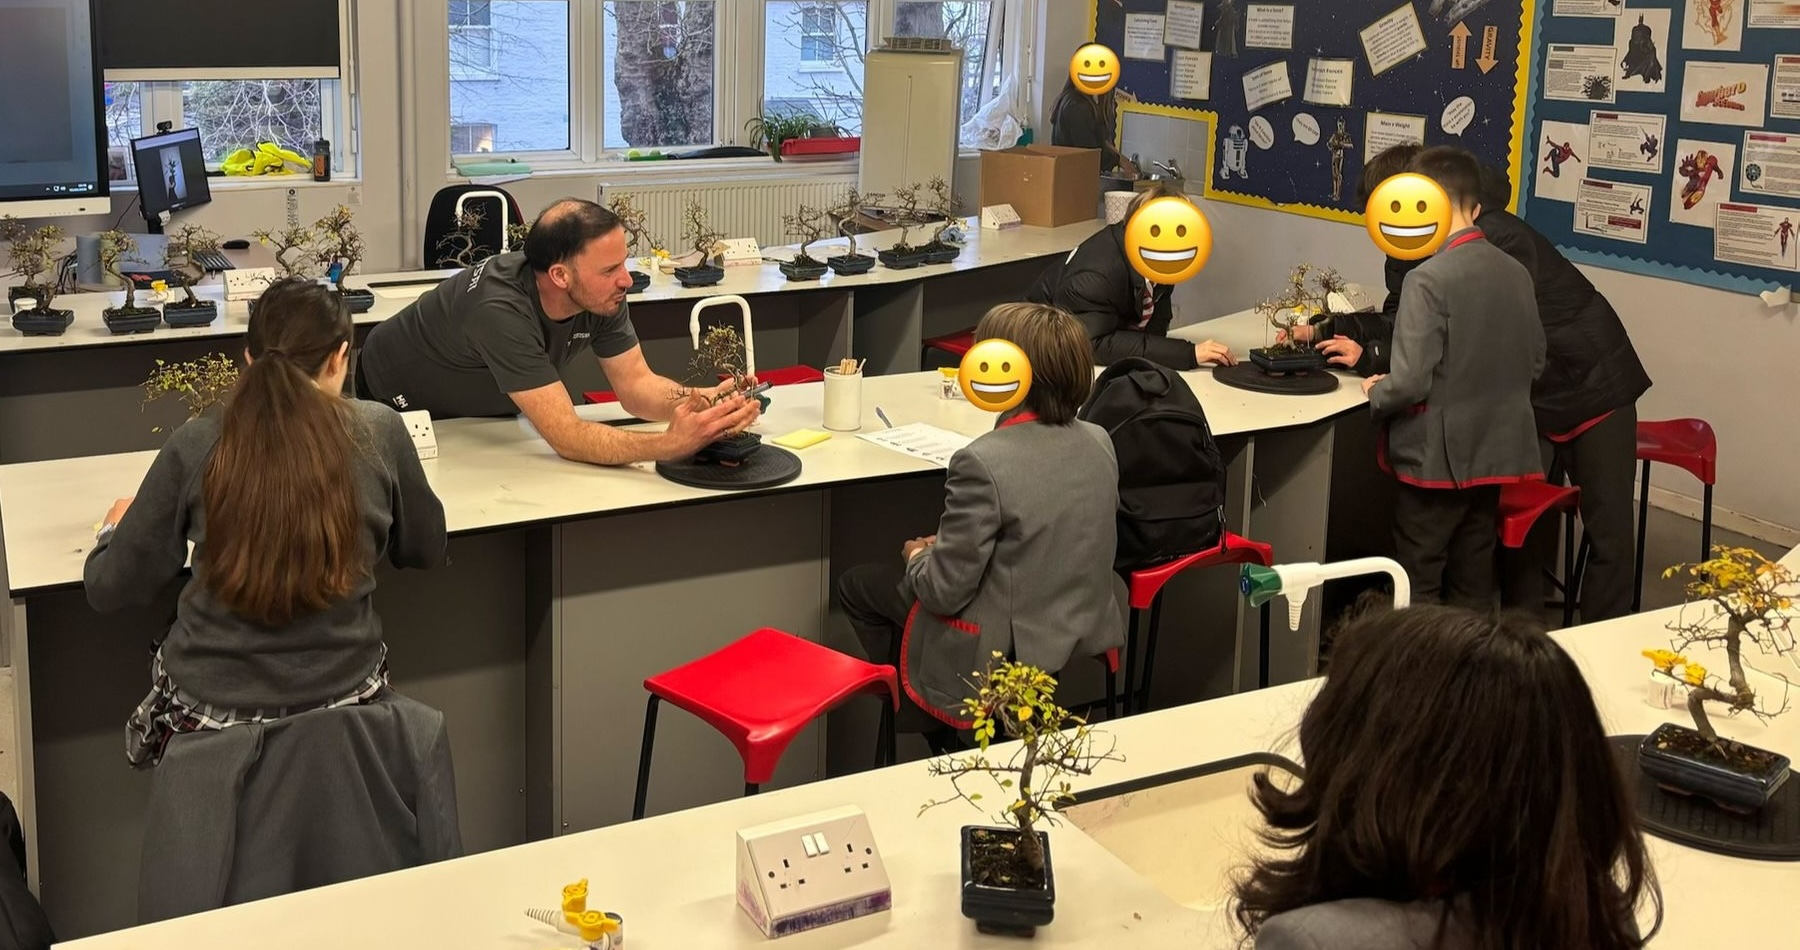
\includegraphics[angle=0,origin=c,width=1.0\textwidth]{2026_01/res/2601_kids_school}
        \centerline{\emph{Liz with her prize-winning Shishigashira Maple.}}
    \end{minipage}
\end{center}

\begin{center}$\cdots$\end{center}

\noindent
\textit{Got a bonsai\--related rumour, quirky story, or fun fact?}\\
\textit{Share it with us for the next edition of \textit{Potting Shed Gossip}!}
\closearticle
\clearpage
